\section{Tyrimo rezultatai}
\label{sec:tyrimo_rezultatai}

Šiame skyriuje pateikiami penki tyrimai – architektūros, \textit{Dropout} tikimybės, paketinio normalizavimo, aktyvacijos funkcijos ir optimizavimo algoritmo įtaka mokymo bei validavimo metrikoms. Visiems tyrimams naudojama:
\begin{itemize}
    \item Vaizdams – \texttt{subset\_ratio}~$=0{,}2$ ($1\,182$ vaizdų), kad tyrimai įsitenka į turimus skaičiavimo resursus.
    \item Laiko eilutėms – pilna $1\,500$ įrašų aibė ($30$ klasių, $50$ įrašų klasei).
    \item Kiekvienas eksperimentas mokomas $20$ epochų su \texttt{batch\_size}~$=64$, \texttt{learning\_rate}~$=10^{-3}$.
    \item Kiekvienoje lentelėje pateikiami: geriausios epochos validavimo tikslumas (\texttt{val\_acc}) ir paklaida (\texttt{val\_loss}) bei testavimo tikslumas (\texttt{test\_acc}). Geriausias kiekvieno tyrimo variantas paryškintas.
\end{itemize}

\subsection{Architektūros įtaka}
\label{subsec:rez_architektura}

Lyginamos trys konvoliucinių blokų konfigūracijos kiekvienai užduočiai (žr.~\ref{tab:rez_architektura} lentelę). Validavimo metrikų kitimas per epochas pateiktas \ref{fig:rez_architektura_image} ir~\ref{fig:rez_architektura_keystroke} pav.

\begin{table}[H]
    \centering
    \caption{Architektūros tyrimo rezultatai. Geriausi variantai paryškinti.}
    \begin{tabular}{|l|l|c|c|c|}
        \hline
        Užduotis & Variantas & \texttt{val\_acc} & \texttt{val\_loss} & \texttt{test\_acc} \\
        \hline
        \multirow{3}{*}{Vaizdai}
            & Small \texttt{(16, 32)}        & $0{,}8254$ & $0{,}4955$ & $0{,}8305$ \\ \cline{2-5}
            & \textbf{Medium \texttt{(32, 64, 128)}} & $\mathbf{0{,}8413}$ & $\mathbf{0{,}8387}$ & $0{,}8178$ \\ \cline{2-5}
            & \textbf{Large \texttt{(64, 128, 256)}} & $0{,}8201$ & $0{,}4792$ & $\mathbf{0{,}8432}$ \\
        \hline
        \multirow{3}{*}{Laiko eilutės}
            & Small \texttt{(32,)}           & $0{,}6792$ & $1{,}5507$ & $0{,}7467$ \\ \cline{2-5}
            & \textbf{Medium \texttt{(64, 128)}} & $\mathbf{0{,}6917}$ & $\mathbf{1{,}0635}$ & $0{,}7200$ \\ \cline{2-5}
            & Large \texttt{(64, 128, 256)}  & $0{,}6042$ & $1{,}4302$ & $0{,}6233$ \\
        \hline
    \end{tabular}
    \label{tab:rez_architektura}
\end{table}


\begin{figure}[H]
    \centering
    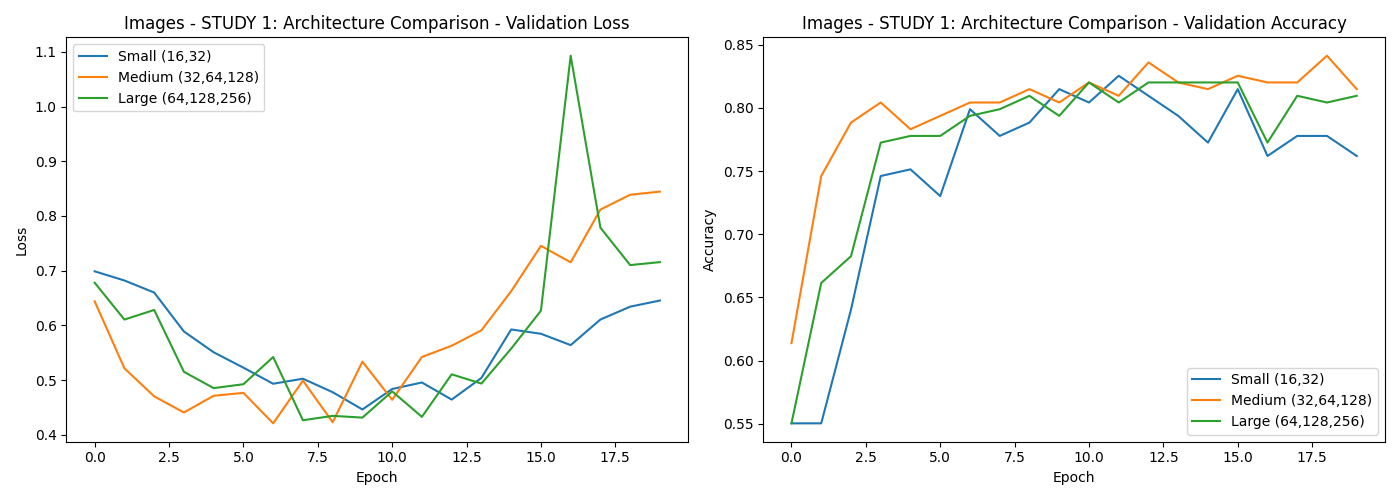
\includegraphics[width=0.9\linewidth]{3Lab/results/architecture/img_comparison.png}
    \caption{Architektūros tyrimas – vaizdų užduotis}
    \label{fig:rez_architektura_image}
\end{figure}

\begin{figure}[H]
    \centering
    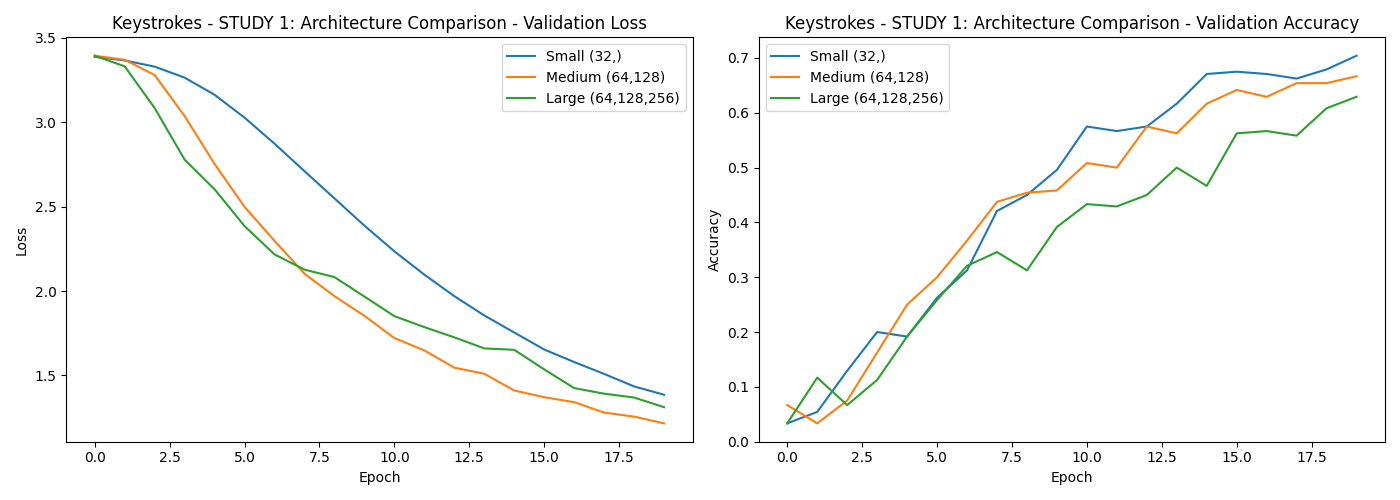
\includegraphics[width=0.9\linewidth]{3Lab/results/architecture/ks_comparison.png}
    \caption{Architektūros tyrimas – laiko eilučių užduotis}
    \label{fig:rez_architektura_keystroke}
\end{figure}

Pastebimi rezultatai:
\begin{itemize}
    \item Vaizdams \textbf{vidutinė architektūra} \texttt{(32, 64, 128)} pasiekė didžiausią validavimo tikslumą ($0{,}8413$), tačiau didžiausias \texttt{test\_acc} ($0{,}8432$) buvo gautas su \textbf{didele} \texttt{(64, 128, 256)} architektūra – tai rodo, kad gilesnis tinklas geriau generalizuoja, nors validavimo aibėje šiek tiek labiau persimokė.
    \item Laiko eilutėms didžiausią validavimo tikslumą gavo \texttt{(64, 128)} architektūra ($0{,}6917$). Dvigubinant filtrų skaičių iki \texttt{(64, 128, 256)} tinklas pradeda sparčiai persimokyti – $1\,500$ įrašų aibei tai per gilus modelis.
\end{itemize}

\subsection{\textit{Dropout} tikimybės įtaka}
\label{subsec:rez_dropout}

Tikrinamos keturios \textit{Dropout} tikimybės: $0$, $0{,}25$, $0{,}5$ ir $0{,}75$. Architektūra pagal nutylėjimą (vaizdams \texttt{(32, 64, 128)}, laiko eilutėms \texttt{(64, 128)}). Rezultatai pateikti~\ref{tab:rez_dropout} lentelėje, validavimo metrikos – \ref{fig:rez_dropout_image} ir~\ref{fig:rez_dropout_keystroke} pav.

\begin{table}[H]
    \centering
    \caption{\textit{Dropout} tikimybės tyrimo rezultatai. Geriausi variantai paryškinti.}
    \begin{tabular}{|l|l|c|c|c|}
        \hline
        Užduotis & Tikimybė & \texttt{val\_acc} & \texttt{val\_loss} & \texttt{test\_acc} \\
        \hline
        \multirow{4}{*}{Vaizdai}
            & \textbf{$0{,}00$} & $\mathbf{0{,}8466}$ & $0{,}8865$ & $\mathbf{0{,}8347}$ \\ \cline{2-5}
            & $0{,}25$ & $0{,}8095$ & $0{,}4478$ & $0{,}8093$ \\ \cline{2-5}
            & $0{,}50$ & $0{,}7989$ & $\mathbf{0{,}4459}$ & $0{,}7924$ \\ \cline{2-5}
            & $0{,}75$ & $0{,}6667$ & $0{,}6780$ & $0{,}5763$ \\
        \hline
        \multirow{4}{*}{Laiko eilutės}
            & \textbf{$0{,}00$} & $\mathbf{0{,}7125}$ & $\mathbf{0{,}9609}$ & $\mathbf{0{,}7533}$ \\ \cline{2-5}
            & $0{,}25$ & $0{,}6750$ & $1{,}1523$ & $0{,}7167$ \\ \cline{2-5}
            & $0{,}50$ & $0{,}6000$ & $1{,}6406$ & $0{,}6767$ \\ \cline{2-5}
            & $0{,}75$ & $0{,}0917$ & $3{,}3900$ & $0{,}0600$ \\
        \hline
    \end{tabular}
    \label{tab:rez_dropout}
\end{table}


\begin{figure}[H]
    \centering
    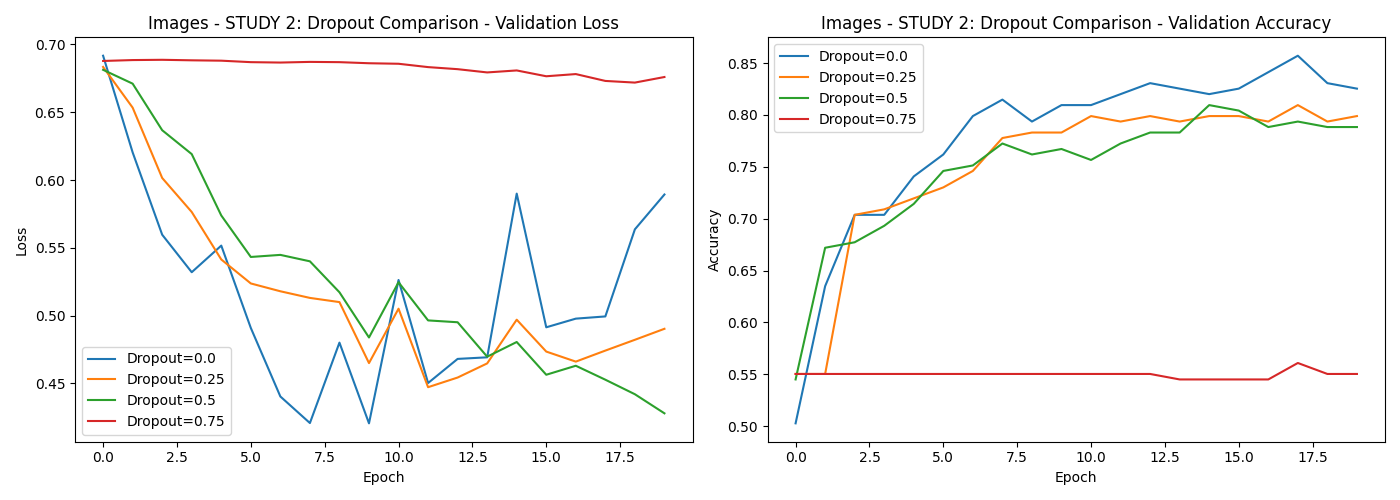
\includegraphics[width=0.9\linewidth]{3Lab/results/dropout/img_comparison.png}
    \caption{\textit{Dropout} tyrimas – vaizdų užduotis}
    \label{fig:rez_dropout_image}
\end{figure}

\begin{figure}[H]
    \centering
    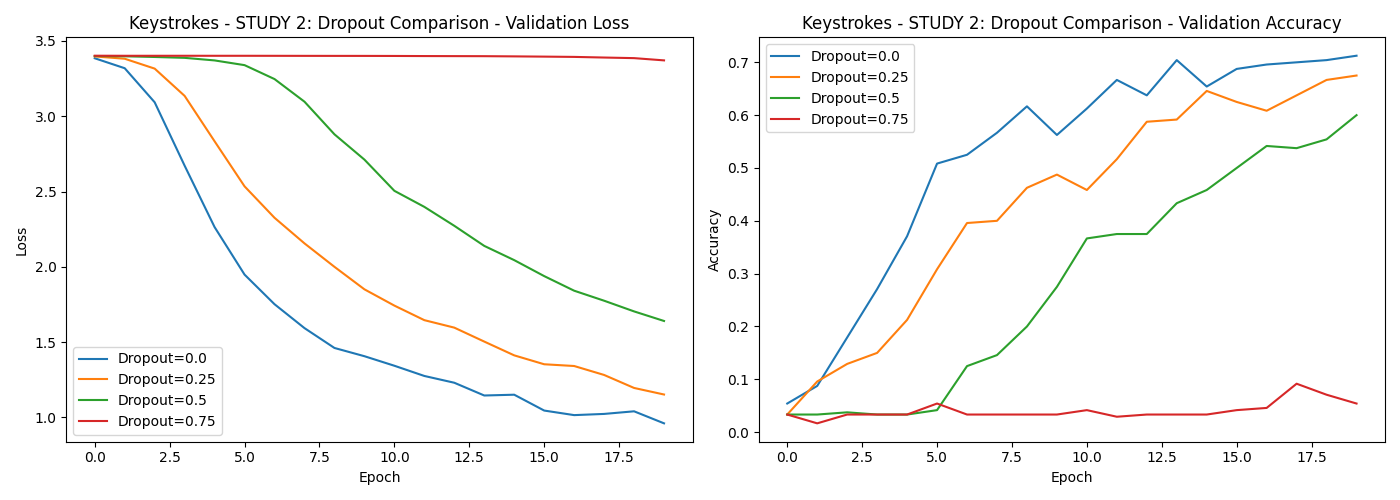
\includegraphics[width=0.9\linewidth]{3Lab/results/dropout/ks_comparison.png}
    \caption{\textit{Dropout} tyrimas – laiko eilučių užduotis}
    \label{fig:rez_dropout_keystroke}
\end{figure}

Pastebimi rezultatai:
\begin{itemize}
    \item Abiem užduotims \textbf{tikimybė $0{,}0$} davė geriausią validavimo tikslumą, nes mokymo aibės yra nedidelės ir tinklas nepasiekia stipraus persimokymo. Padidinus tikimybę iki $0{,}5$ tikslumas krenta, bet ne katastrofiškai.
    \item \textbf{Tikimybė $0{,}75$} sunaikina mokymo signalą – laiko eilučių modelis nepasiekia net $10\,\%$ tikslumo (kas yra atsitiktinio spėjimo lygis $30$ klasių užduotyje).
    \item Vaizdams su \texttt{Dropout}~$=0{,}5$ \texttt{val\_loss} ($0{,}4459$) yra mažiausias, todėl jei svarbi prognozės pasitikėjimo kalibracija, ši tikimybė geriausia – tačiau kelia mažesnį tikslumą.
\end{itemize}

\subsection{Paketinio normalizavimo įtaka}
\label{subsec:rez_batch_norm}

Lyginamos dvi konfigūracijos – tinklas su paketinio normalizavimo (\textit{batch normalization}, BN) sluoksniais ir be jų. Rezultatai pateikti~\ref{tab:rez_batch_norm} lentelėje, validavimo metrikos – \ref{fig:rez_batch_norm_image} ir~\ref{fig:rez_batch_norm_keystroke} pav.

\begin{table}[H]
    \centering
    \caption{Paketinio normalizavimo tyrimo rezultatai. Geriausi variantai paryškinti.}
    \begin{tabular}{|l|l|c|c|c|}
        \hline
        Užduotis & Variantas & \texttt{val\_acc} & \texttt{val\_loss} & \texttt{test\_acc} \\
        \hline
        \multirow{2}{*}{Vaizdai}
            & Be BN     & $0{,}8360$ & $0{,}6696$ & $0{,}8432$ \\ \cline{2-5}
            & \textbf{Su BN} & $\mathbf{0{,}8942}$ & $\mathbf{0{,}3272}$ & $\mathbf{0{,}8602}$ \\
        \hline
        \multirow{2}{*}{Laiko eilutės}
            & Be BN     & $0{,}6750$ & $1{,}2623$ & $0{,}7167$ \\ \cline{2-5}
            & \textbf{Su BN} & $\mathbf{0{,}9167}$ & $\mathbf{0{,}2516}$ & $\mathbf{0{,}9033}$ \\
        \hline
    \end{tabular}
    \label{tab:rez_batch_norm}
\end{table}


\begin{figure}[H]
    \centering
    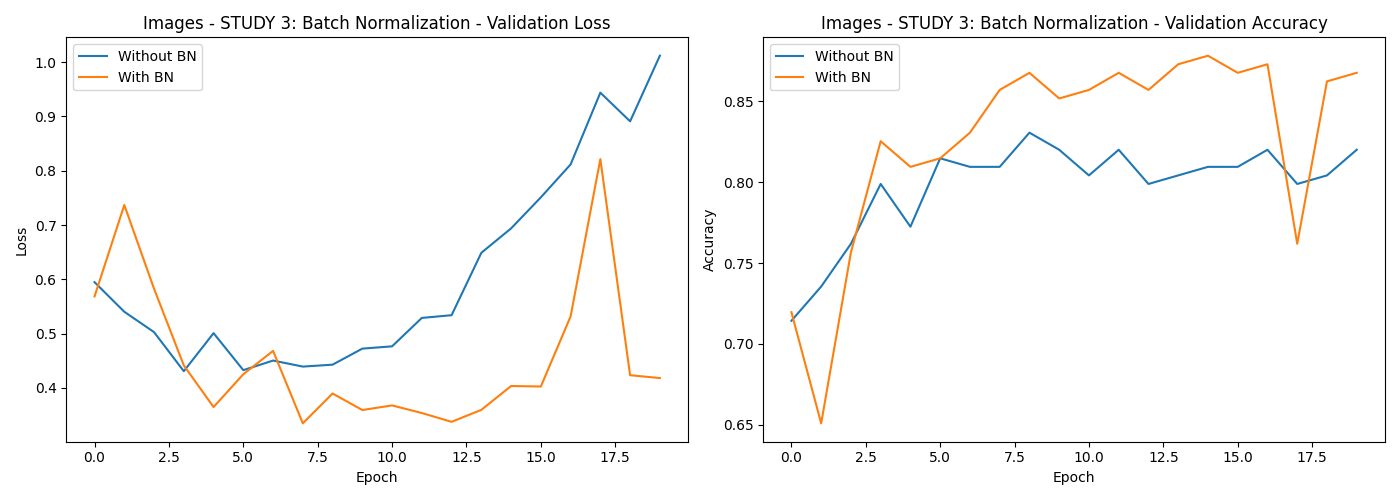
\includegraphics[width=0.9\linewidth]{3Lab/results/batch_norm/img_comparison.png}
    \caption{Paketinio normalizavimo tyrimas – vaizdų užduotis}
    \label{fig:rez_batch_norm_image}
\end{figure}

\begin{figure}[H]
    \centering
    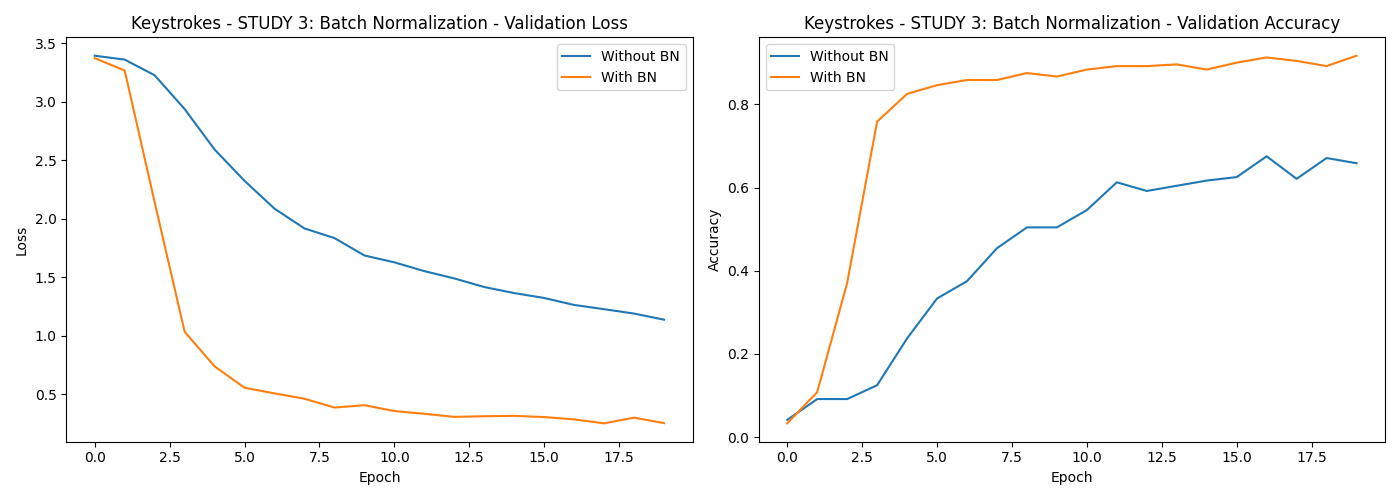
\includegraphics[width=0.9\linewidth]{3Lab/results/batch_norm/ks_comparison.png}
    \caption{Paketinio normalizavimo tyrimas – laiko eilučių užduotis}
    \label{fig:rez_batch_norm_keystroke}
\end{figure}

Pastebimi rezultatai:
\begin{itemize}
    \item BN sluoksniai \textbf{ryškiai pagerino abu modelius}: vaizdų \texttt{val\_acc} pakilo nuo $0{,}8360$ iki $0{,}8942$, laiko eilučių – nuo $0{,}6750$ iki $0{,}9167$.
    \item Validavimo paklaida sumažėjo apie $2 \times$, o validavimo tikslumas svyruoja gerokai mažiau – BN stabilizuoja mokymo procesą.
    \item Iš visų penkių tyrimų \textbf{BN konfigūracija} pasirodė geriausiai abiem užduotims, todėl ji parinkta galutiniam modelio įvertinimui (\ref{sec:geriausias_modelis} sk.).
\end{itemize}

\subsection{Aktyvacijos funkcijos įtaka}
\label{subsec:rez_aktyvacija}

Lyginamos keturios aktyvacijos funkcijos: \textit{ReLU}, \textit{LeakyReLU} ($\alpha = 0{,}01$), \textit{Tanh} ir \textit{ELU}. Rezultatai pateikti~\ref{tab:rez_aktyvacija} lentelėje, validavimo metrikų kitimas – \ref{fig:rez_aktyvacija_image} ir~\ref{fig:rez_aktyvacija_keystroke} pav.

\begin{table}[H]
    \centering
    \caption{Aktyvacijos funkcijos tyrimo rezultatai. Geriausi variantai paryškinti.}
    \begin{tabular}{|l|l|c|c|c|}
        \hline
        Užduotis & Funkcija & \texttt{val\_acc} & \texttt{val\_loss} & \texttt{test\_acc} \\
        \hline
        \multirow{4}{*}{Vaizdai}
            & \textit{ReLU}        & $0{,}8307$ & $0{,}7279$ & $0{,}8390$ \\ \cline{2-5}
            & \textbf{\textit{LeakyReLU}}  & $0{,}8360$ & $\mathbf{0{,}4455}$ & $\mathbf{0{,}8517}$ \\ \cline{2-5}
            & \textit{Tanh}        & $0{,}8201$ & $0{,}4460$ & $0{,}7966$ \\ \cline{2-5}
            & \textbf{\textit{ELU}} & $\mathbf{0{,}8413}$ & $0{,}5705$ & $0{,}8008$ \\
        \hline
        \multirow{4}{*}{Laiko eilutės}
            & \textit{ReLU}        & $0{,}6500$ & $1{,}2921$ & $0{,}6533$ \\ \cline{2-5}
            & \textit{LeakyReLU}   & $0{,}7583$ & $0{,}9012$ & $0{,}7800$ \\ \cline{2-5}
            & \textbf{\textit{Tanh}} & $\mathbf{0{,}8000}$ & $\mathbf{0{,}7076}$ & $\mathbf{0{,}8333}$ \\ \cline{2-5}
            & \textit{ELU}         & $0{,}7708$ & $0{,}7677$ & $0{,}8100$ \\
        \hline
    \end{tabular}
    \label{tab:rez_aktyvacija}
\end{table}


\begin{figure}[H]
    \centering
    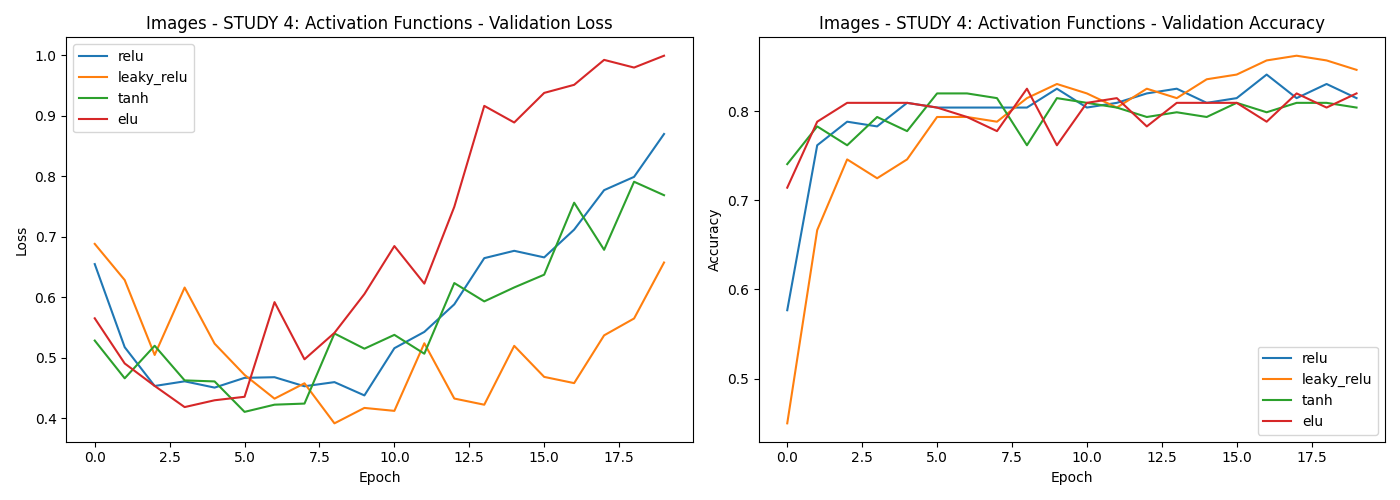
\includegraphics[width=0.9\linewidth]{3Lab/results/activation/img_comparison.png}
    \caption{Aktyvacijos funkcijos tyrimas – vaizdų užduotis}
    \label{fig:rez_aktyvacija_image}
\end{figure}

\begin{figure}[H]
    \centering
    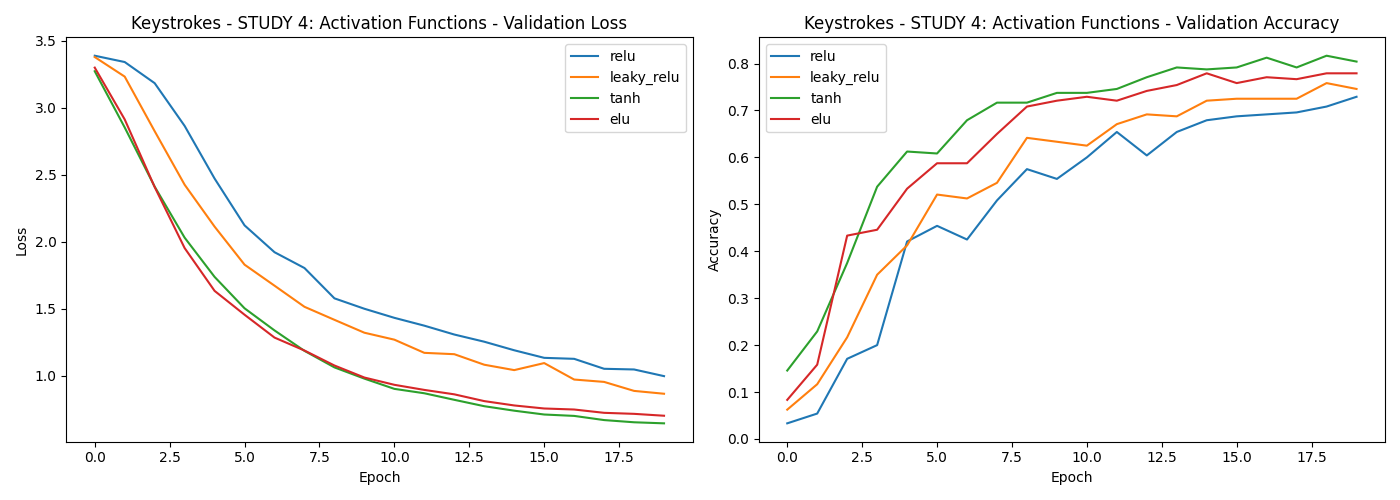
\includegraphics[width=0.9\linewidth]{3Lab/results/activation/ks_comparison.png}
    \caption{Aktyvacijos funkcijos tyrimas – laiko eilučių užduotis}
    \label{fig:rez_aktyvacija_keystroke}
\end{figure}

Pastebimi rezultatai:
\begin{itemize}
    \item Vaizdams visos funkcijos veikia panašiai (\texttt{val\_acc} svyruoja $0{,}82$–$0{,}84$ ribose). Geriausią validavimo tikslumą gavo \textit{ELU}, didžiausią testavimo tikslumą – \textit{LeakyReLU}.
    \item Laiko eilutėms ryškiai išsiskiria \textit{Tanh} – ji geriausiai tinka normalizuotiems $[0,\,1]$ požymiams ($30$ klasių užduotyje pasiekė $\texttt{test\_acc}=0{,}8333$). \textit{ReLU} čia atrodo prasčiausiai – atsineša „mirštančio neurono“ problemą, kai didelė įėjimo verčių dalis yra arti nulio.
\end{itemize}

\subsection{Optimizavimo algoritmo įtaka}
\label{subsec:rez_optimizatorius}

Lyginami keturi optimizavimo algoritmai: \textit{Adam}, \textit{AdamW}, \textit{RMSprop} ir \textit{SGD} (be momentumo). Visų algoritmų \texttt{learning\_rate}~$=10^{-3}$. Rezultatai pateikti~\ref{tab:rez_optimizatorius} lentelėje, validavimo metrikų kitimas – \ref{fig:rez_optimizatorius_image} ir~\ref{fig:rez_optimizatorius_keystroke} pav.

\begin{table}[H]
    \centering
    \caption{Optimizavimo algoritmo tyrimo rezultatai. Geriausi variantai paryškinti.}
    \begin{tabular}{|l|l|c|c|c|}
        \hline
        Užduotis & Algoritmas & \texttt{val\_acc} & \texttt{val\_loss} & \texttt{test\_acc} \\
        \hline
        \multirow{4}{*}{Vaizdai}
            & \textbf{\textit{Adam}}    & $\mathbf{0{,}8466}$ & $0{,}6524$ & $0{,}8347$ \\ \cline{2-5}
            & \textit{SGD}              & $0{,}5503$ & $0{,}6801$ & $0{,}5424$ \\ \cline{2-5}
            & \textbf{\textit{RMSprop}} & $\mathbf{0{,}8466}$ & $0{,}4883$ & $0{,}8390$ \\ \cline{2-5}
            & \textit{AdamW}            & $0{,}8413$ & $\mathbf{0{,}4512}$ & $\mathbf{0{,}8432}$ \\
        \hline
        \multirow{4}{*}{Laiko eilutės}
            & \textit{Adam}             & $0{,}6708$ & $1{,}1537$ & $0{,}7067$ \\ \cline{2-5}
            & \textit{SGD}              & $0{,}0333$ & $3{,}4034$ & $0{,}0333$ \\ \cline{2-5}
            & \textbf{\textit{RMSprop}} & $\mathbf{0{,}7042}$ & $\mathbf{1{,}1310}$ & $\mathbf{0{,}7300}$ \\ \cline{2-5}
            & \textit{AdamW}            & $0{,}6833$ & $1{,}1355$ & $0{,}7200$ \\
        \hline
    \end{tabular}
    \label{tab:rez_optimizatorius}
\end{table}


\begin{figure}[H]
    \centering
    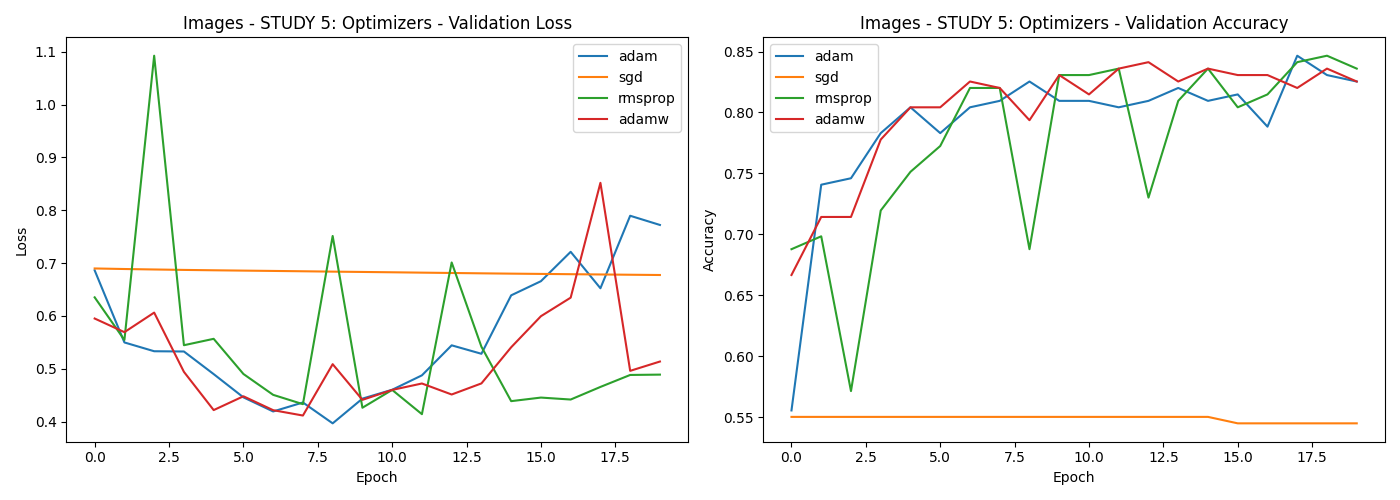
\includegraphics[width=0.9\linewidth]{3Lab/results/optimizer/img_comparison.png}
    \caption{Optimizavimo algoritmo tyrimas – vaizdų užduotis}
    \label{fig:rez_optimizatorius_image}
\end{figure}

\begin{figure}[H]
    \centering
    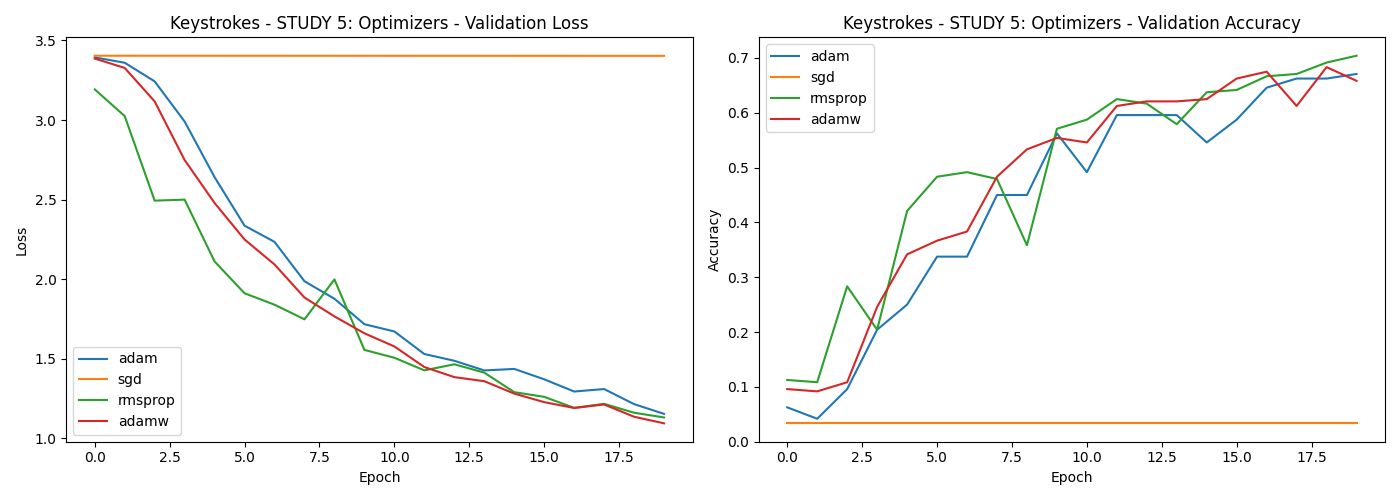
\includegraphics[width=0.9\linewidth]{3Lab/results/optimizer/ks_comparison.png}
    \caption{Optimizavimo algoritmo tyrimas – laiko eilučių užduotis}
    \label{fig:rez_optimizatorius_keystroke}
\end{figure}

Pastebimi rezultatai:
\begin{itemize}
    \item \textit{Adam}, \textit{AdamW} ir \textit{RMSprop} gauna labai panašius rezultatus, nes visi naudoja adaptyvų mokymosi greitį pagal kiekvieno svorio gradiento istoriją.
    \item \textit{SGD} su tokia pačia $10^{-3}$ vertė ryškiai atsilieka – ypač $30$ klasių laiko eilučių užduotyje, kur \texttt{test\_acc}~$=0{,}0333$ (atsitiktinis spėjimas). Kad \textit{SGD} dirbtų konkurencingai, reikėtų paskaičiuoti tinkamą \texttt{learning\_rate} ir/arba pridėti momentumą.
    \item Pagal numatytąsias hiperparametrų reikšmes \textit{Adam} išlieka saugus pasirinkimas abiem užduotims.
\end{itemize}

